\section{Durchführung}

\subsection{Messung der Filterkurve}
Zunächst wird die Güte des Selektivverstärkers untersucht. Dafür wird der Selektivverstärkers mit einem Synthesizer und Oszilloskop bei Frequenzen $\nu = \SI{20}{\kilo\hertz}$ und
$\SI{40}{\kilo\hertz}$ durchgemessen. Die Werte der Messung sind in \autoref{tab:selektiv} gelistet.

\subsection{Messung der Suszeptibilität ausgewählter Stoffe} 
Für den Aufbau der Messbrücke wird der Aufbau nach \autoref{fig:bruecke} aufgebaut. Zusätzlich wird der Frequenzfilter nach \autoref{fig:block} verschaltet.
\begin{figure} [H]
    \centering
    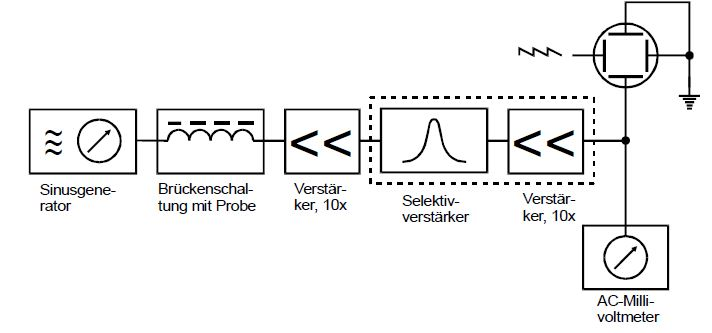
\includegraphics[scale=0.75]{Bilder/Blockschaltbild.jpg}
    \caption{Blockschaltbild. \cite{V606}}
    \label{fig:block}
\end{figure}

\noindent
Untersucht werden die Elemente $\symup{Dy_2O_3}$ und $\symup{Gd_2O_3}$.
Zuerst wird die Brücke zuerst ohne Probe abgeglichen und dann wird die Probe eingeführt und die Spannung notiert und die Brücke wird erneut abgeglichen. Dies wird für jede
Probe 3mal wiederholt. Bei jedem Abgleich wird der Widerstand und die Spannung notiert.


